\section{Extra-Credit: Panorama}

These are the results I got with the given images.
I noticed that a black region appears to the right of the warped
right-image. I couldn't figure out why this was the case,
especially since it does not occur when I use my own images.
But the panorama still looks accurate.

\begin{figure}[H]
  \centering
  \begin{minipage}{0.39\textwidth}
    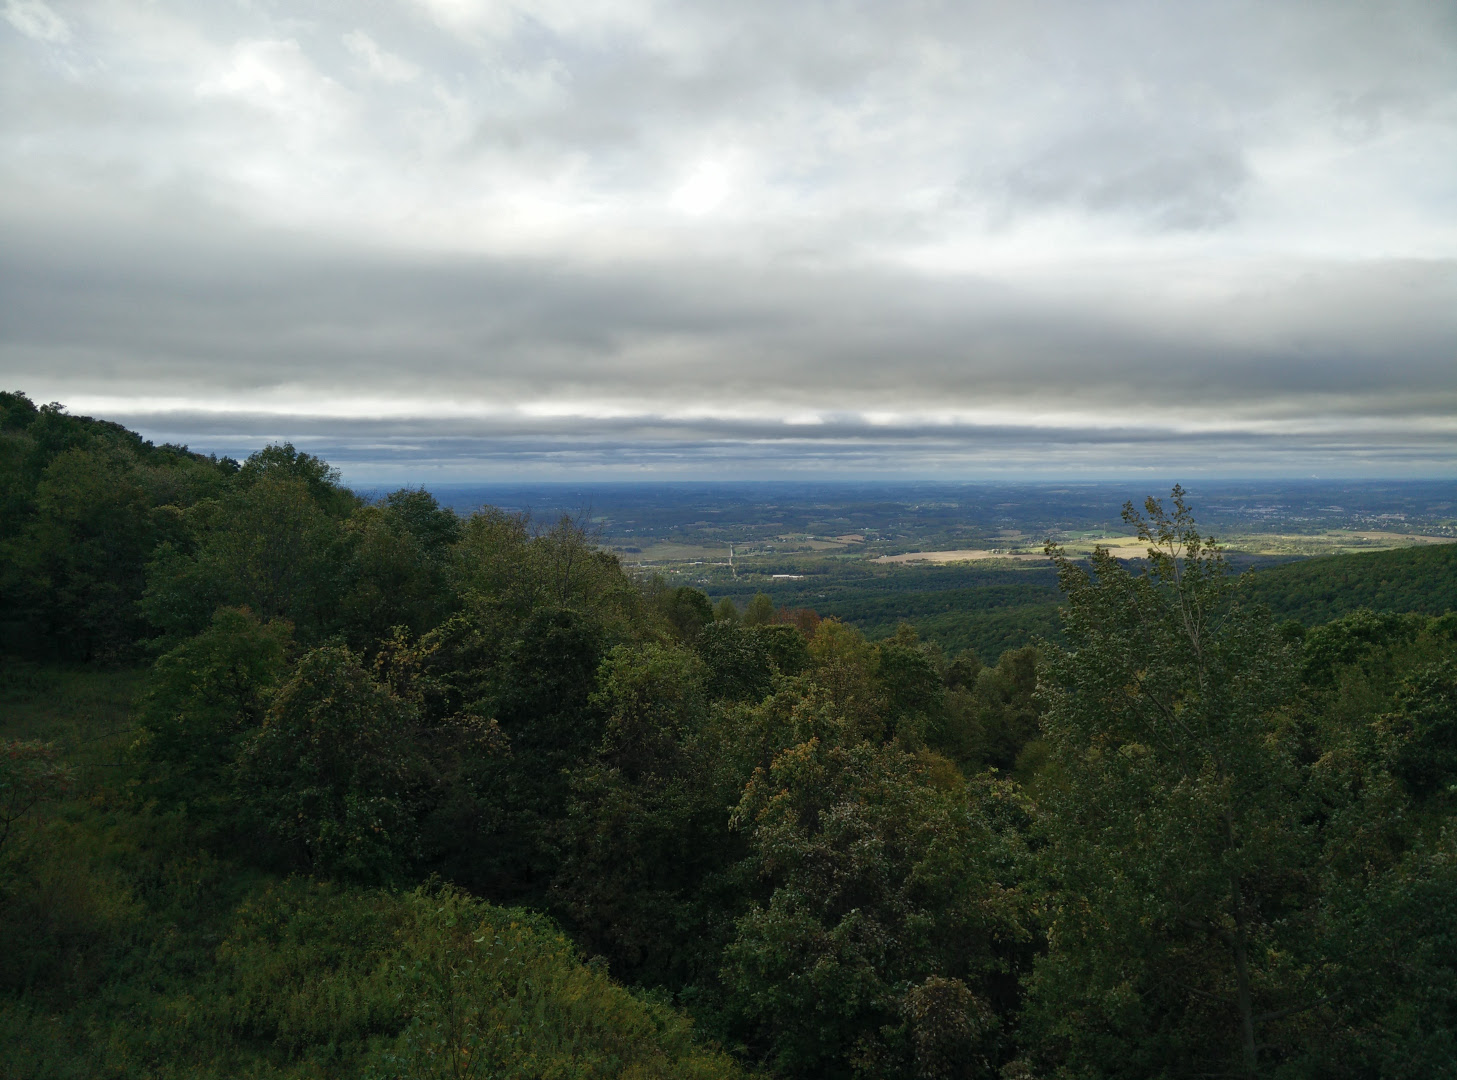
\includegraphics[width=\textwidth]{images/given-left.jpg}
    \caption{Given Left Image}
    \label{fig:left-image}
  \end{minipage}
  \hfill
  \begin{minipage}{0.39\textwidth}
    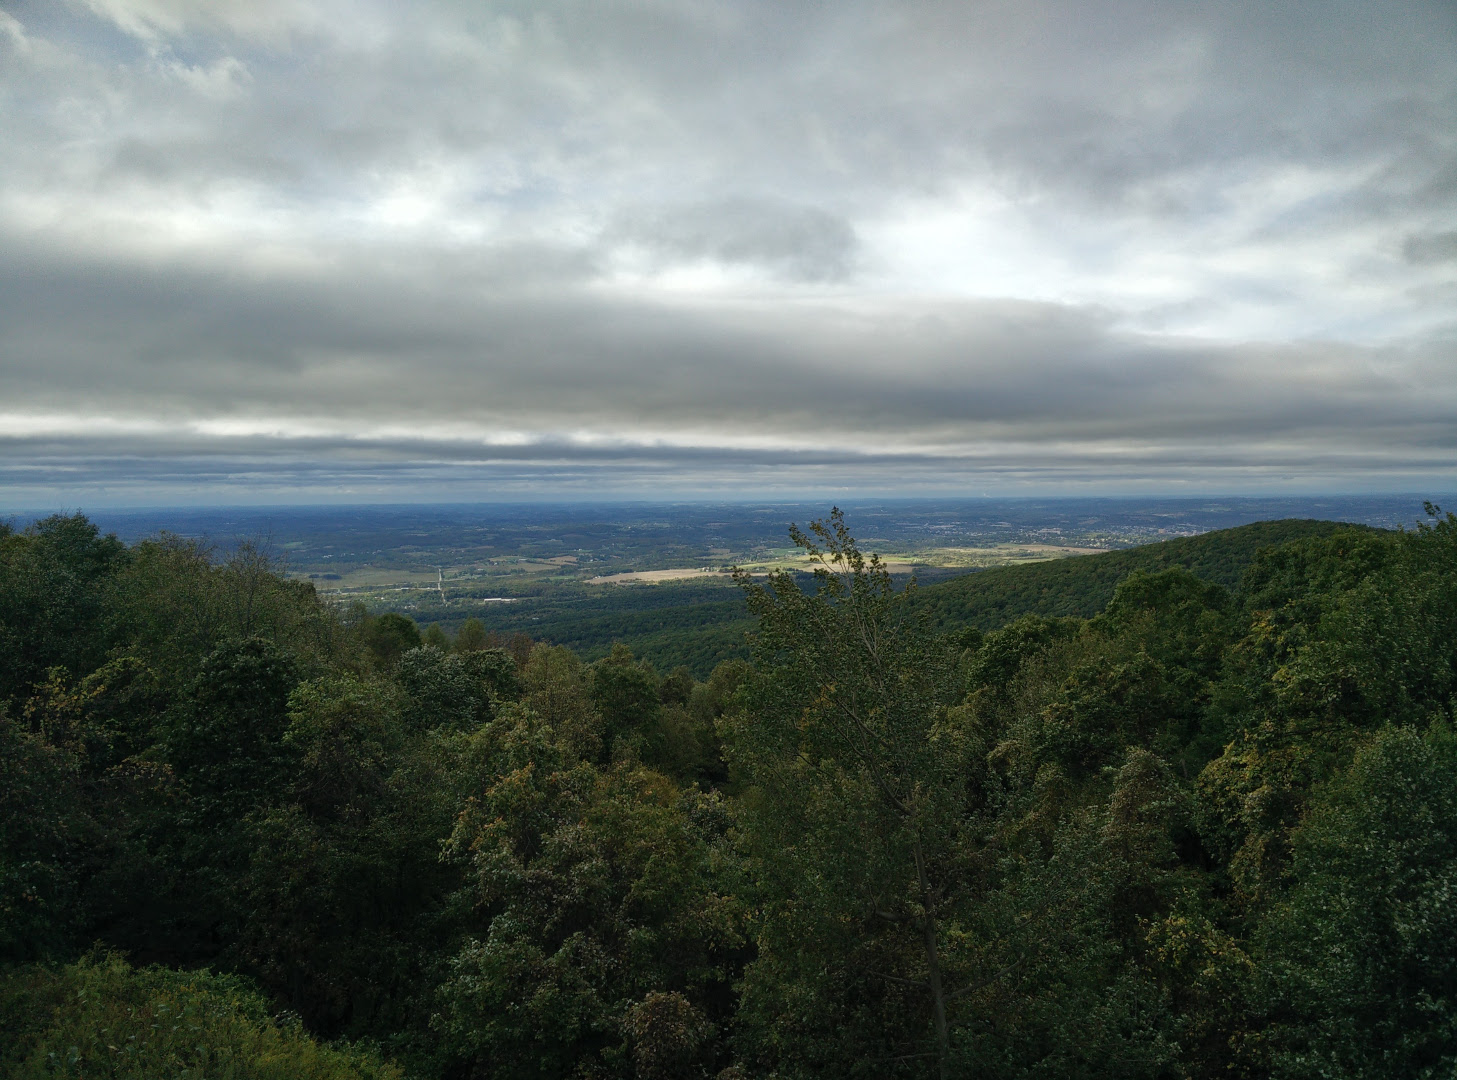
\includegraphics[width=\textwidth]{images/given-right.jpg}
    \caption{Given Right Image}
    \label{fig:right-image}
  \end{minipage}
  \hfill
  \begin{minipage}{0.89\textwidth}
    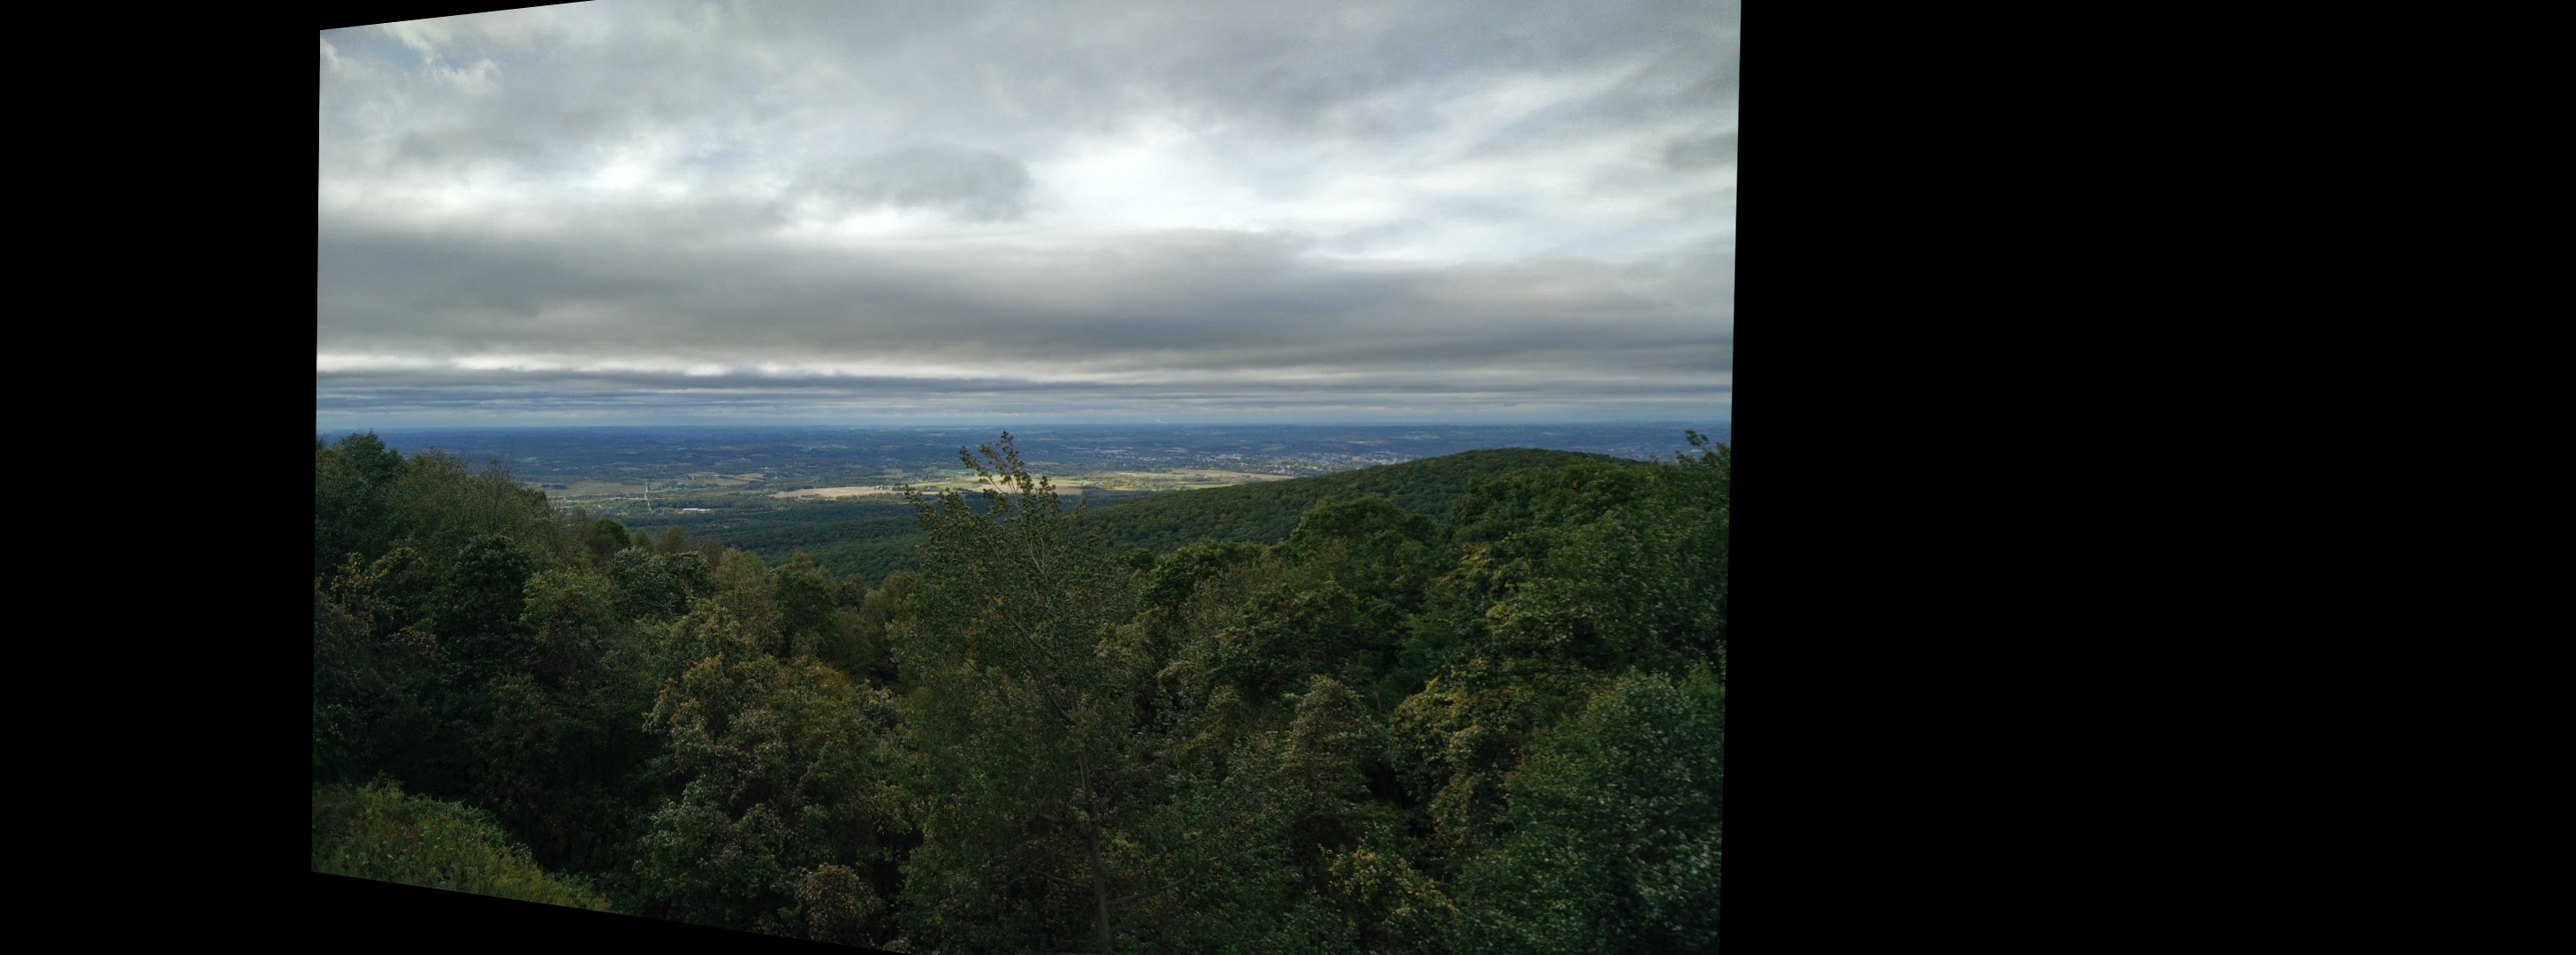
\includegraphics[width=\textwidth]{images/warped-right-0.jpg}
    \caption{Right Warped to Left}
    \label{fig:cv-desk}
  \end{minipage}
  \hfill
  \begin{minipage}{0.89\textwidth}
    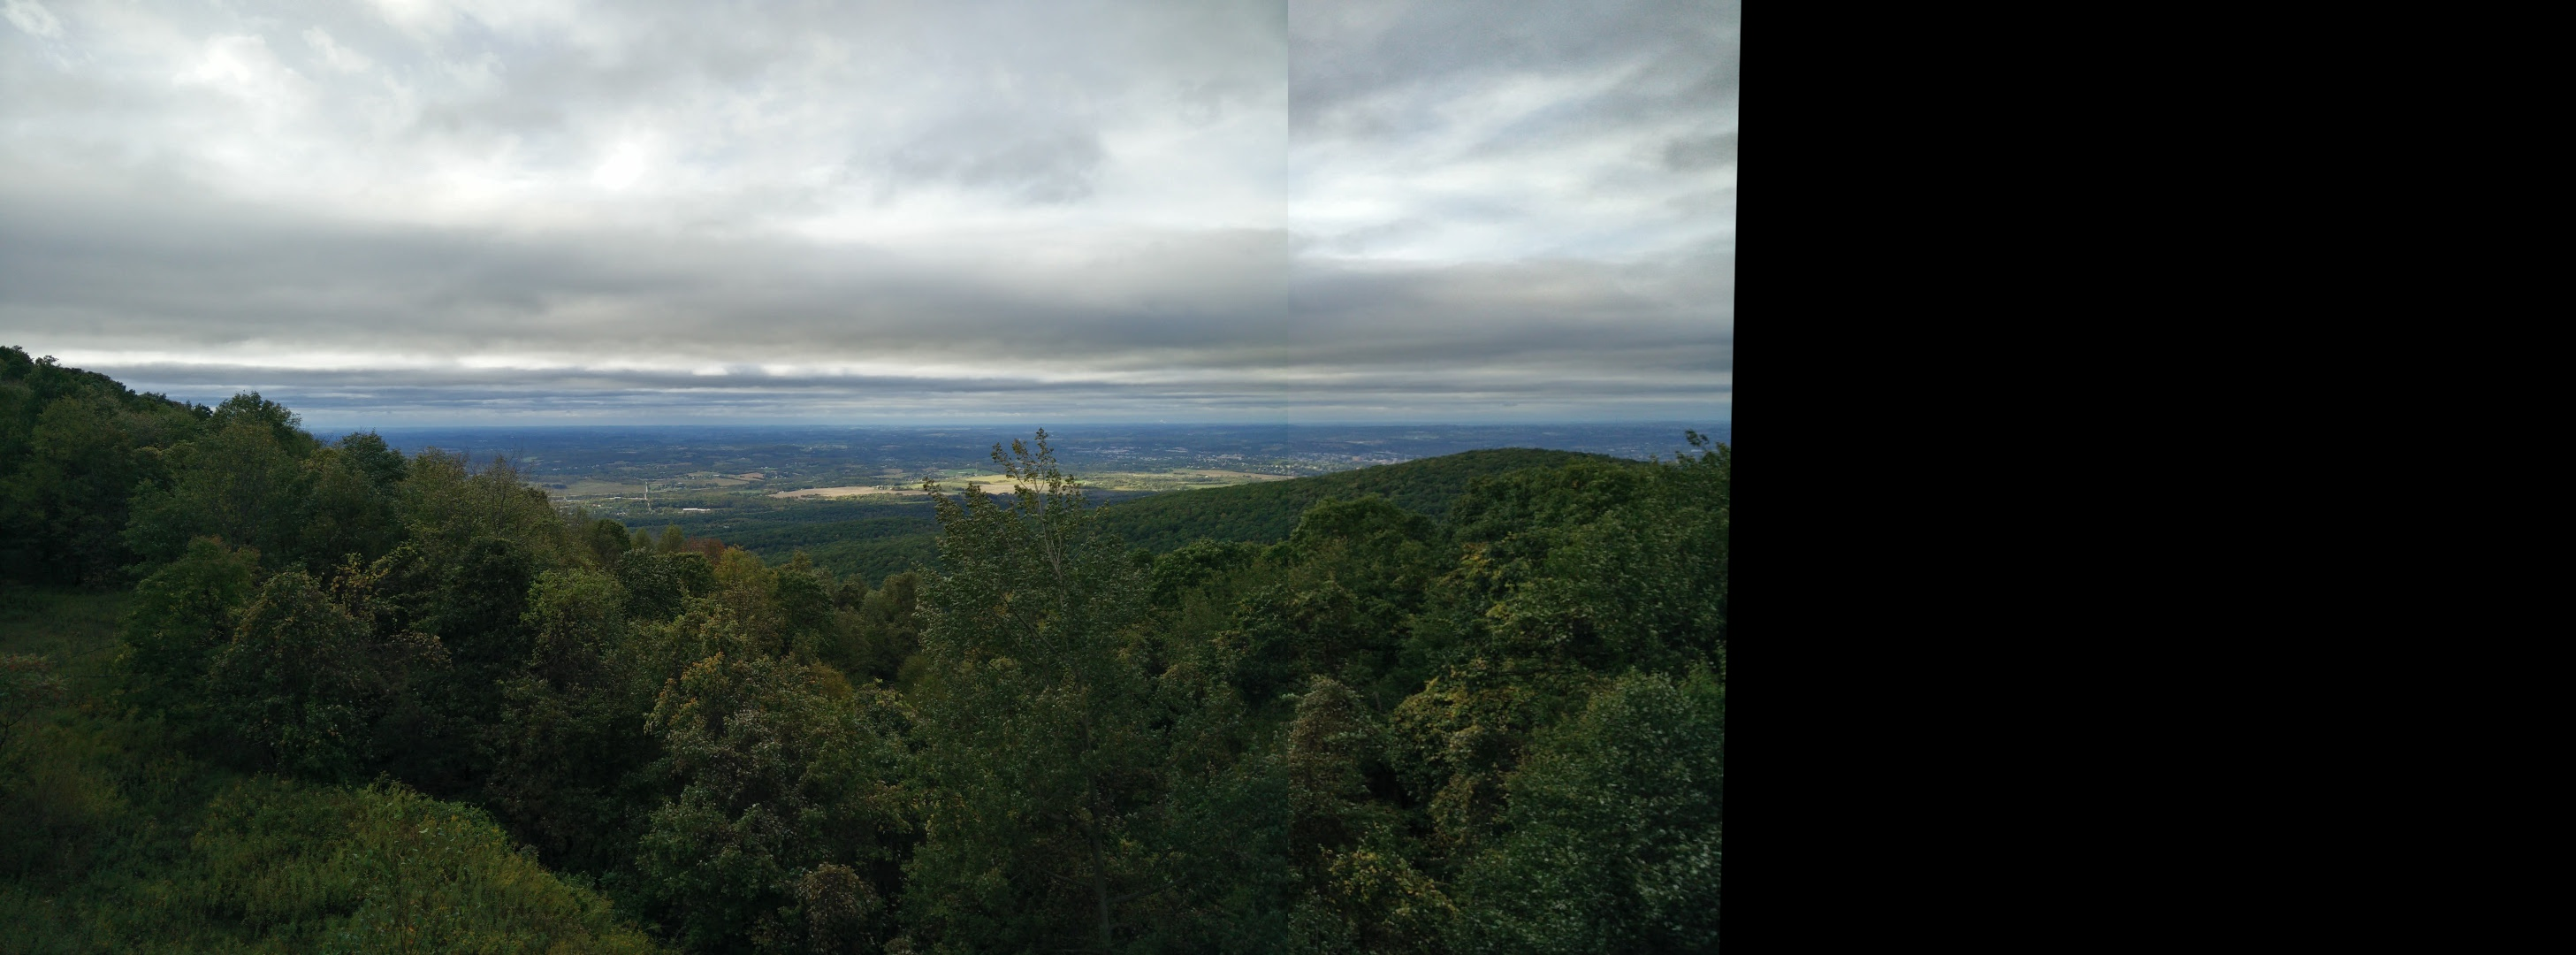
\includegraphics[width=\textwidth]{images/panorama-0.jpg}
    \caption{Left-Right}
    \label{fig:hp-desk}
  \end{minipage}
\end{figure}

\newpage
These are the results I got using my own images.
I tried to be a bit creative and stitch together three images
by recursively warping the right image to the middle image,
and then warping the (middle + right) image to the left image.

\begin{figure}[H]
  \centering
  \begin{minipage}{0.29\textwidth}
    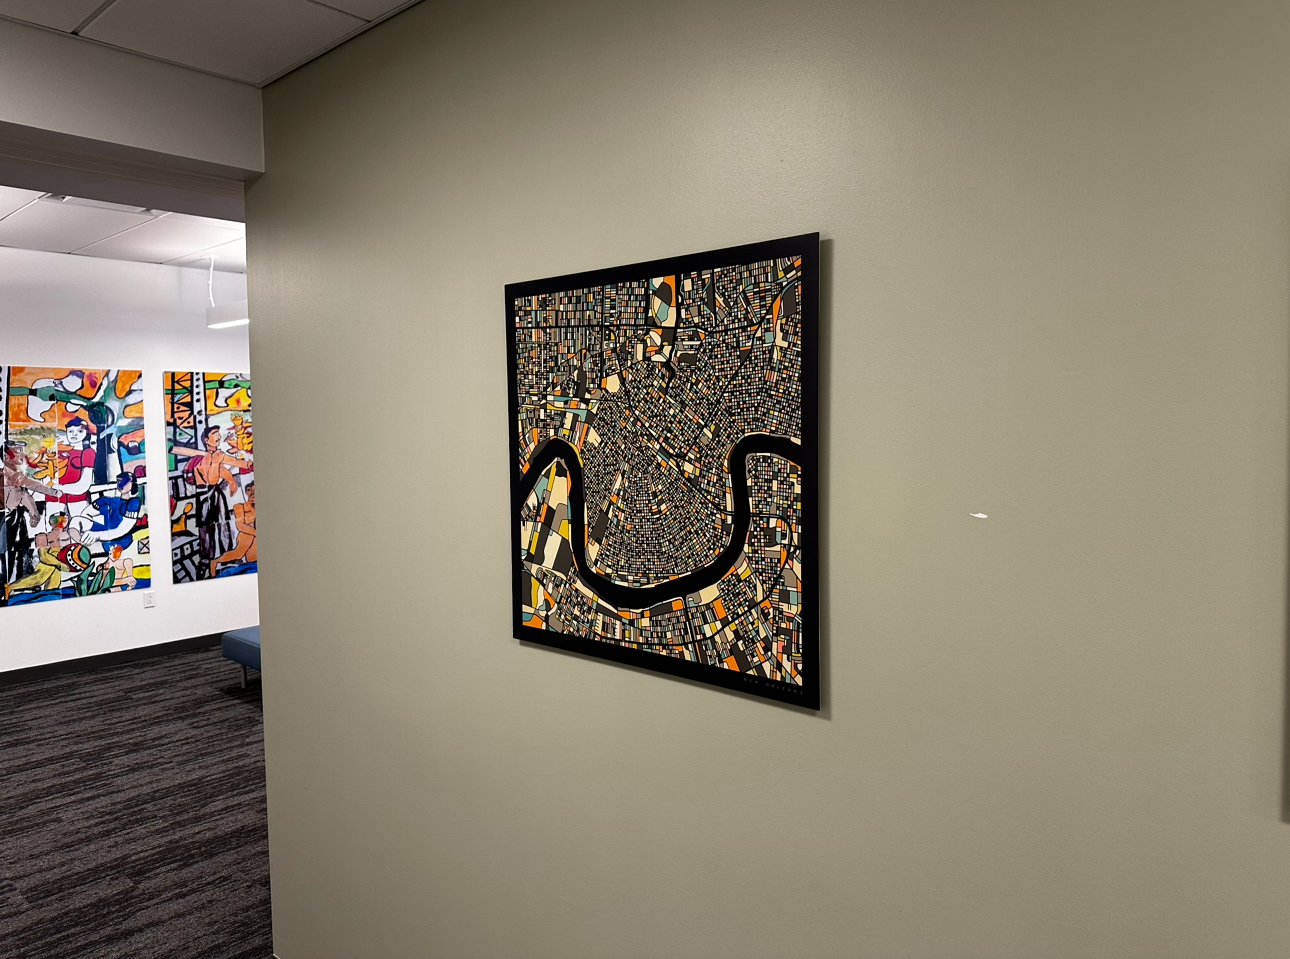
\includegraphics[width=\textwidth]{images/left.jpg}
    \caption{Left}
    \label{fig:cv-cover}
  \end{minipage}
  \hfill
  \begin{minipage}{0.29\textwidth}
    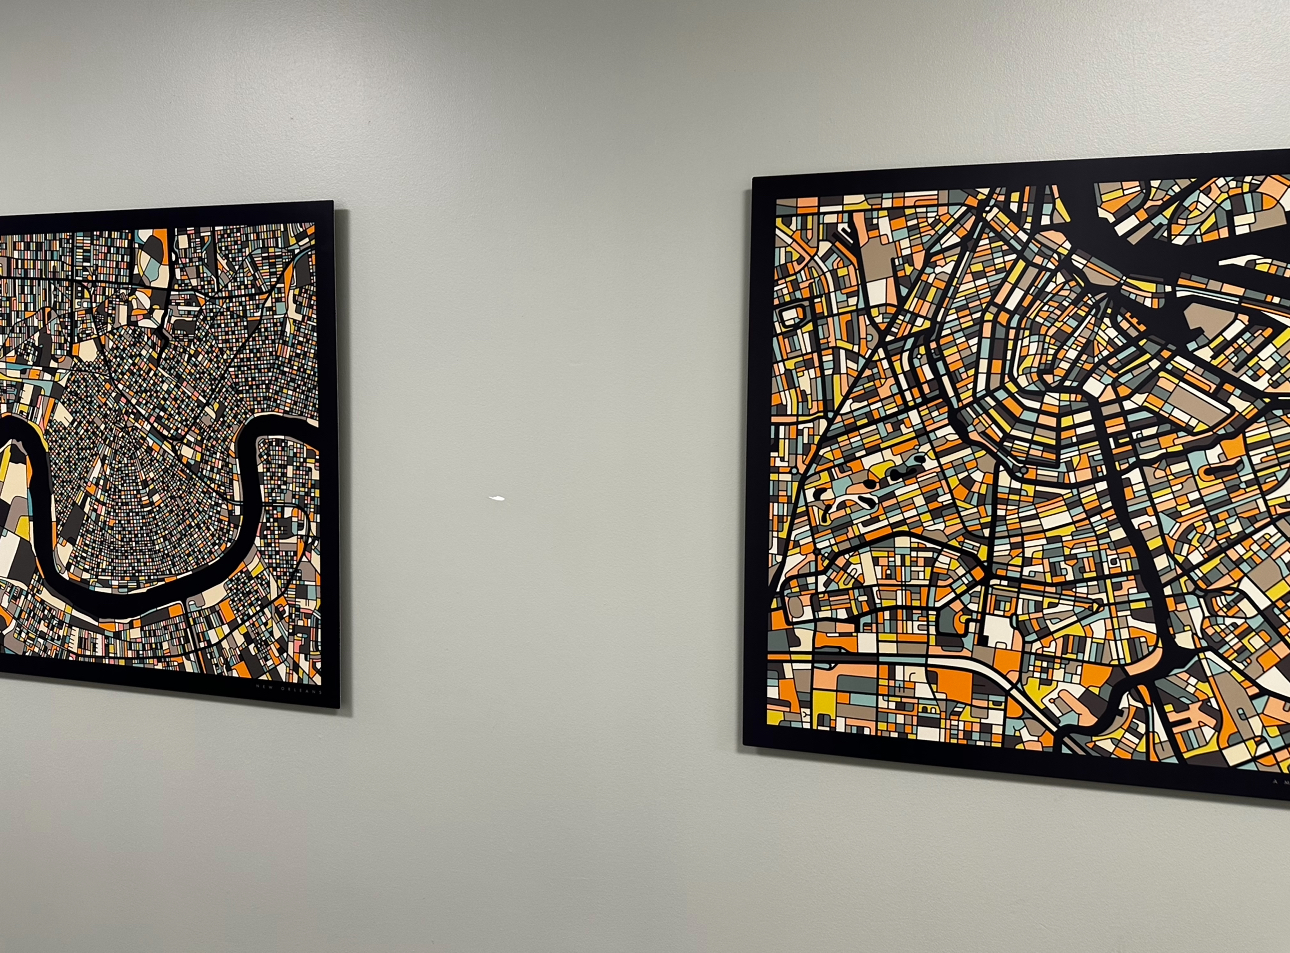
\includegraphics[width=\textwidth]{images/middle.jpg}
    \caption{Middle}
    \label{fig:hp-cover}
  \end{minipage}
  \hfill
  \begin{minipage}{0.29\textwidth}
    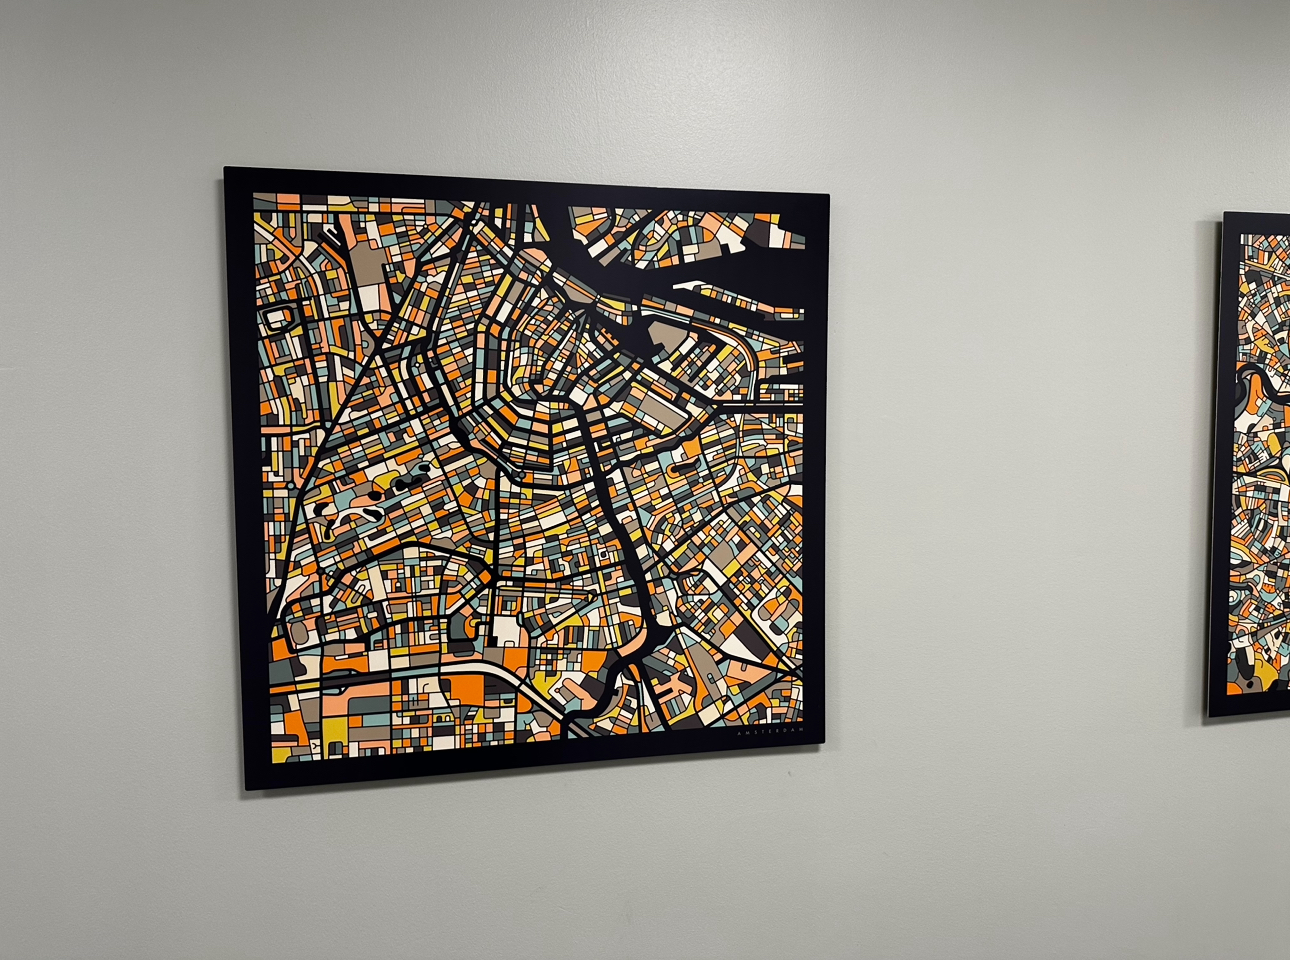
\includegraphics[width=\textwidth]{images/right.jpg}
    \caption{Right}
    \label{fig:hp-cover}
  \end{minipage}
\end{figure}

% left and middle
% \newpage
\textbf{Left composed with Middle}
\begin{figure}[H]
  \centering
  \begin{minipage}{0.79\textwidth}
    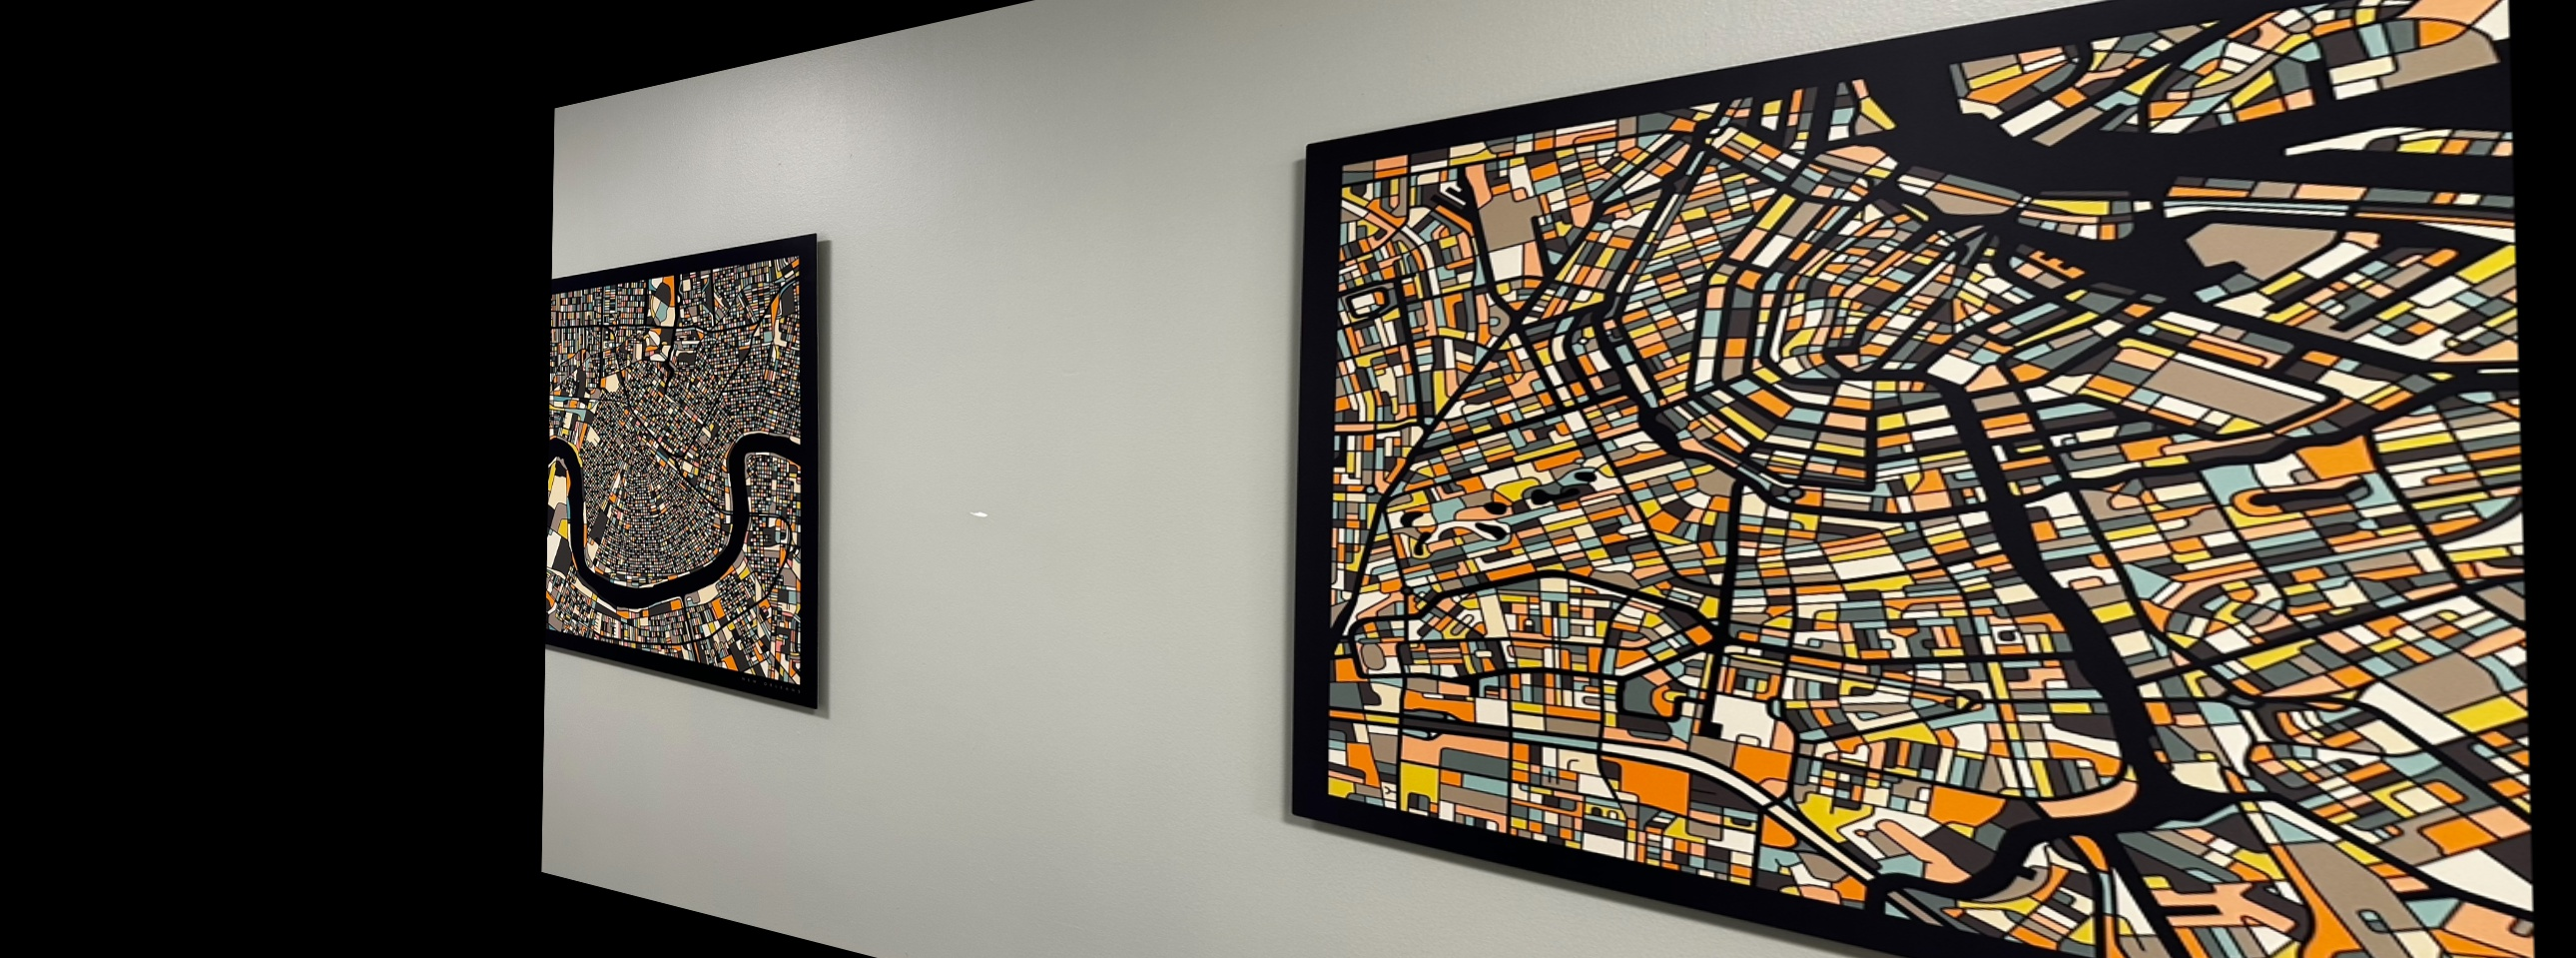
\includegraphics[width=\textwidth]{images/warped-right-1.jpg}
    \caption{Middle Warped to Left}
    \label{fig:cv-desk}
  \end{minipage}
  \hfill
  \begin{minipage}{0.79\textwidth}
    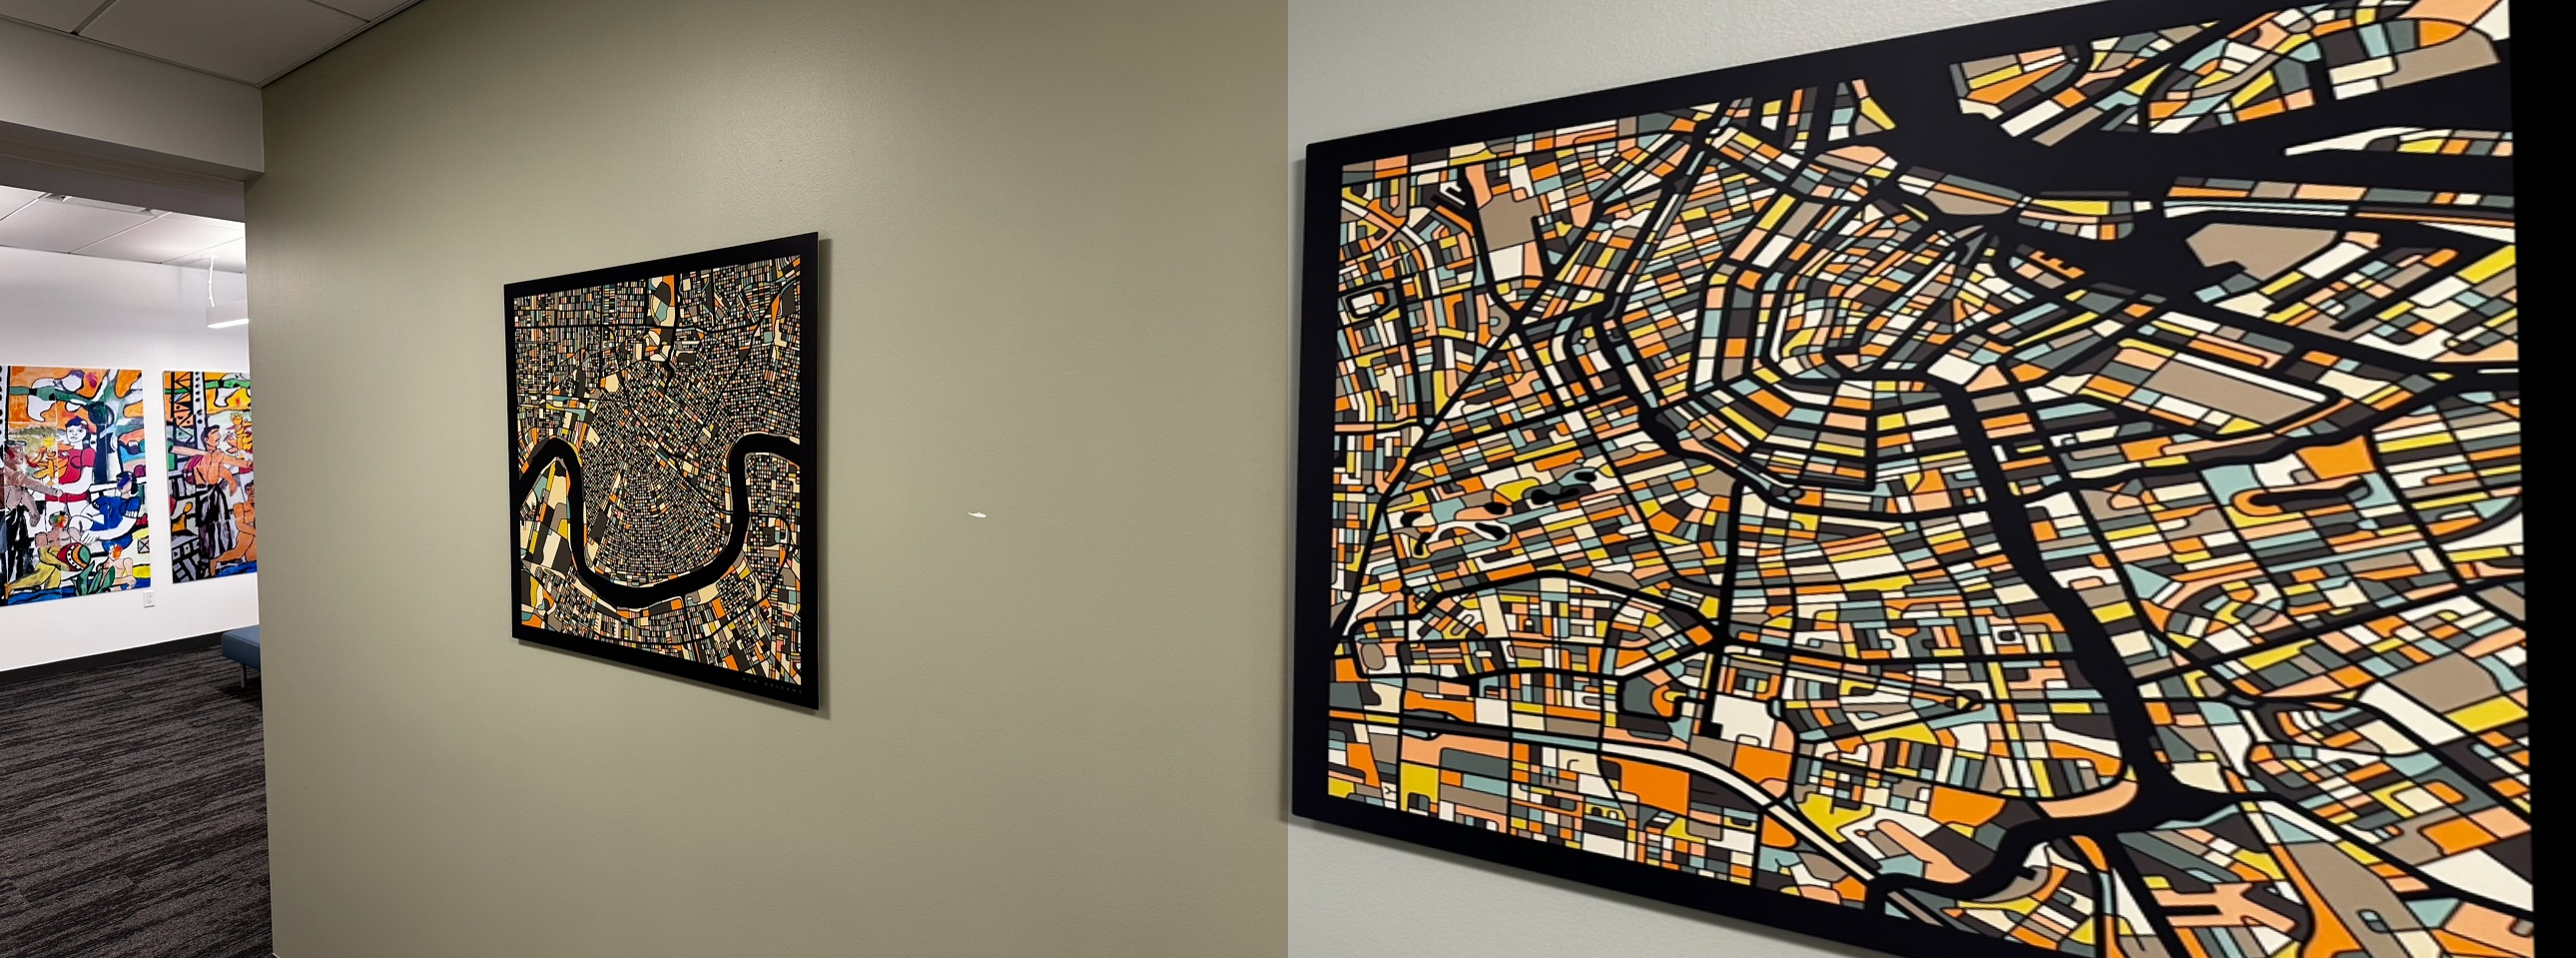
\includegraphics[width=\textwidth]{images/panorama-1.jpg}
    \caption{Left + Middle}
    \label{fig:hp-desk}
  \end{minipage}
\end{figure}

\step
\emph{
  It is noticeable that the camera captured the two images with
  slightly different color temperatures.
  Still, the panorama looks accurate.
}

% middle and right
\newpage
\textbf{Middle composed with Right}
\begin{figure}[H]
  \centering
  \begin{minipage}{0.79\textwidth}
    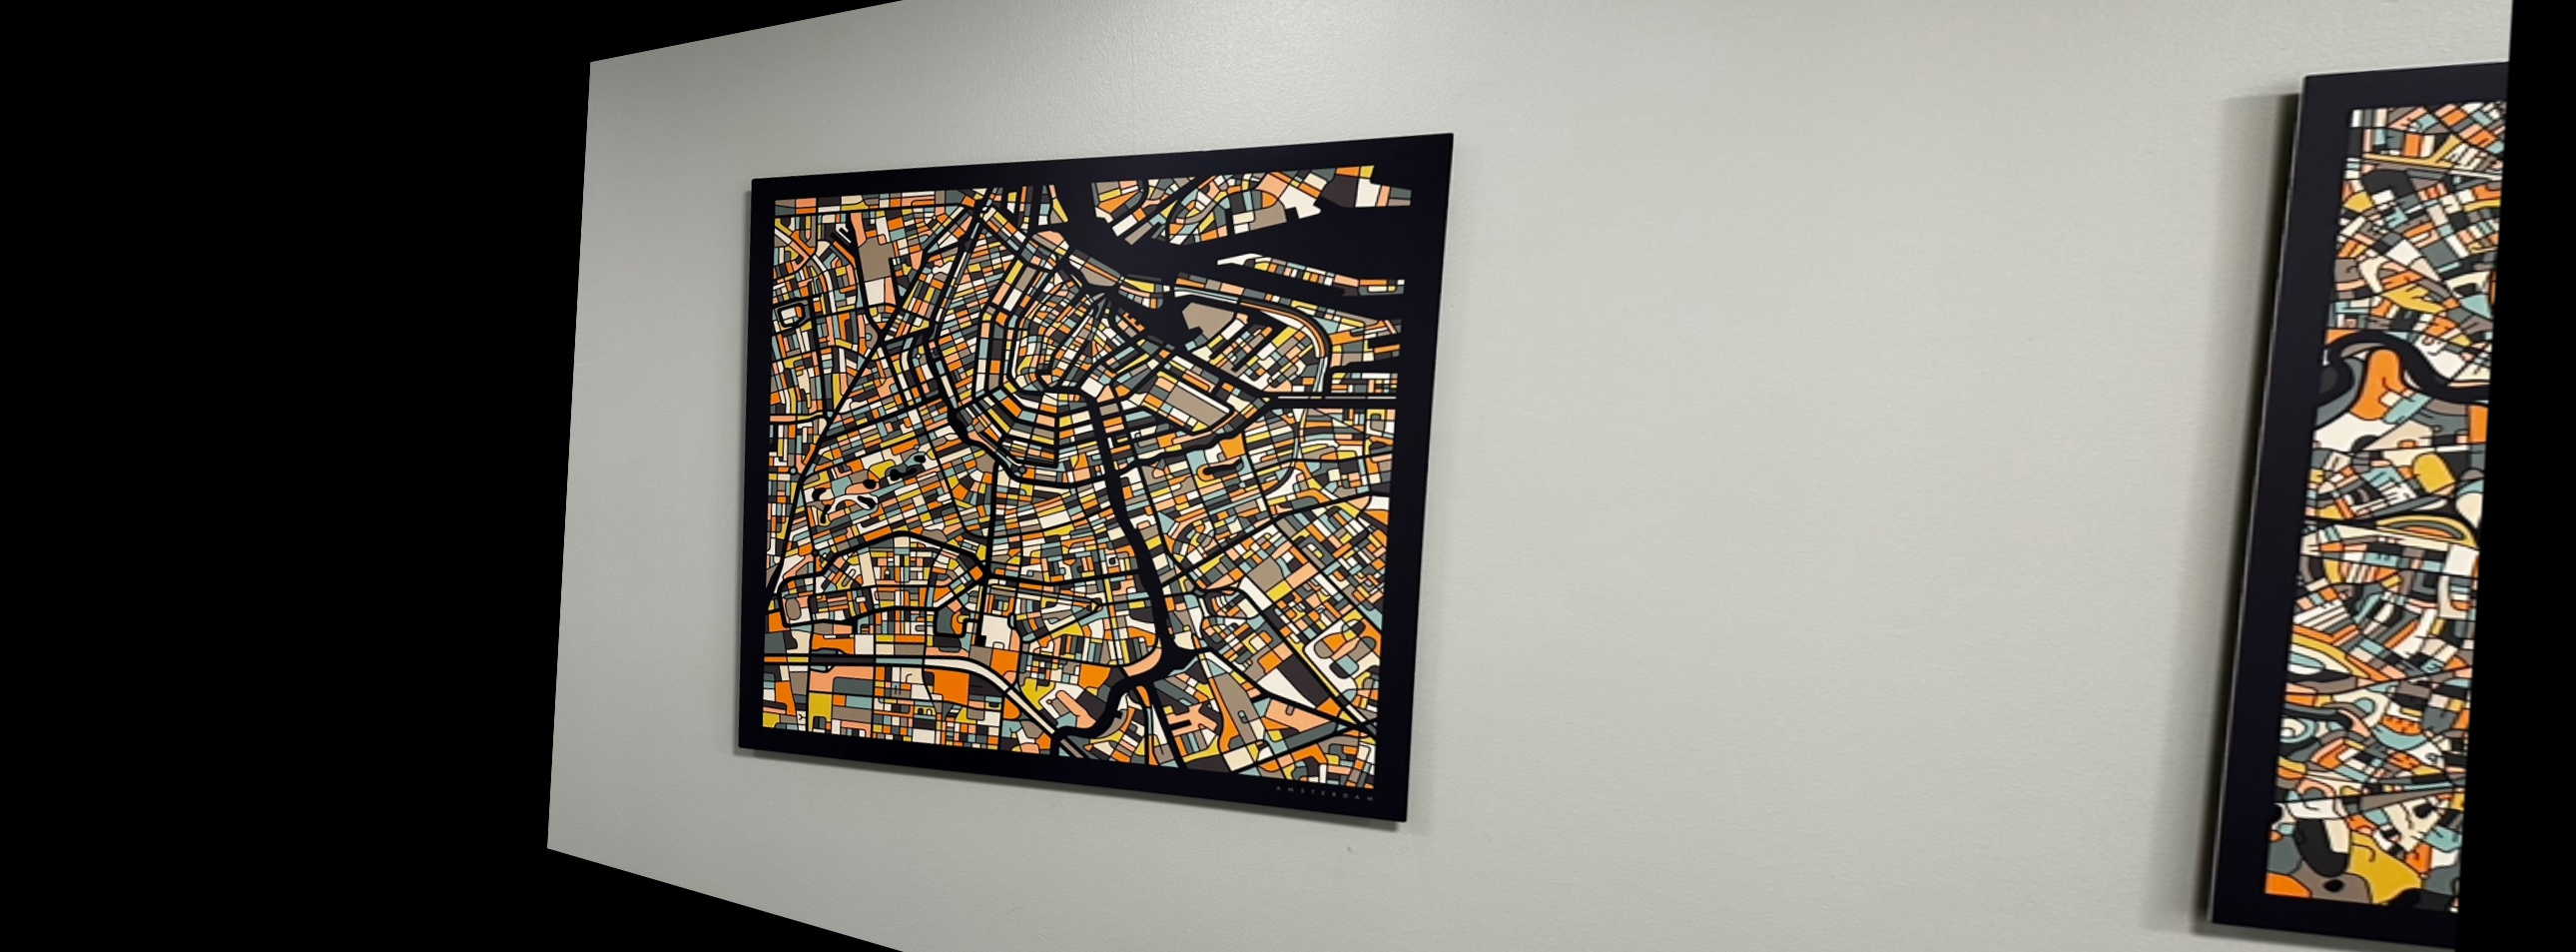
\includegraphics[width=\textwidth]{images/warped-right-2.jpg}
    \caption{Right Warped to Middle}
    \label{fig:cv-desk}
  \end{minipage}
  \hfill
  \begin{minipage}{0.79\textwidth}
    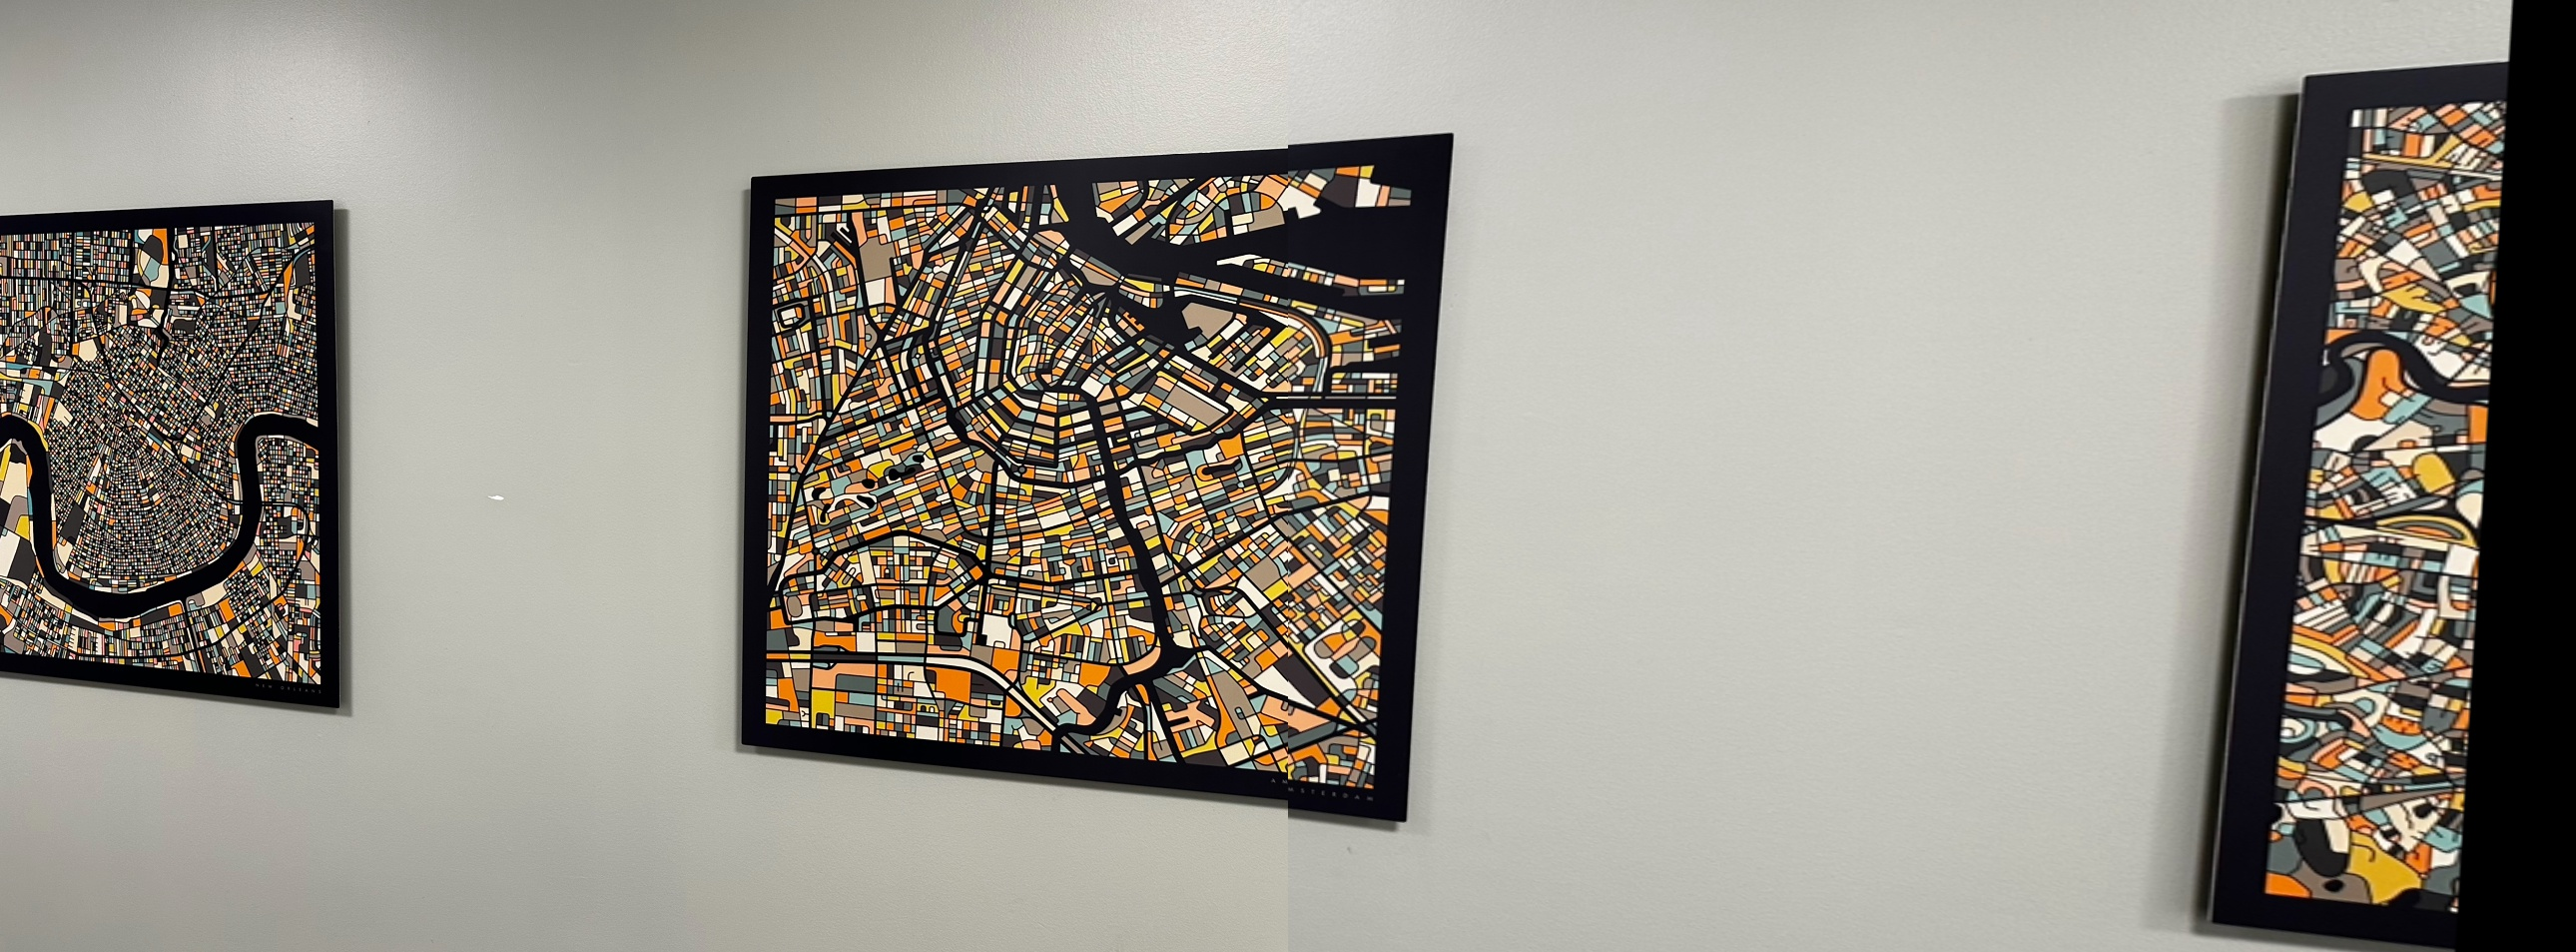
\includegraphics[width=\textwidth]{images/panorama-2.jpg}
    \caption{Middle + Right}
    \label{fig:hp-desk}
  \end{minipage}
\end{figure}

% left and middle-right
\newpage
\textbf{Left composed with Middle + Right}
\begin{figure}[H]
  \centering
  \begin{minipage}{\textwidth}
    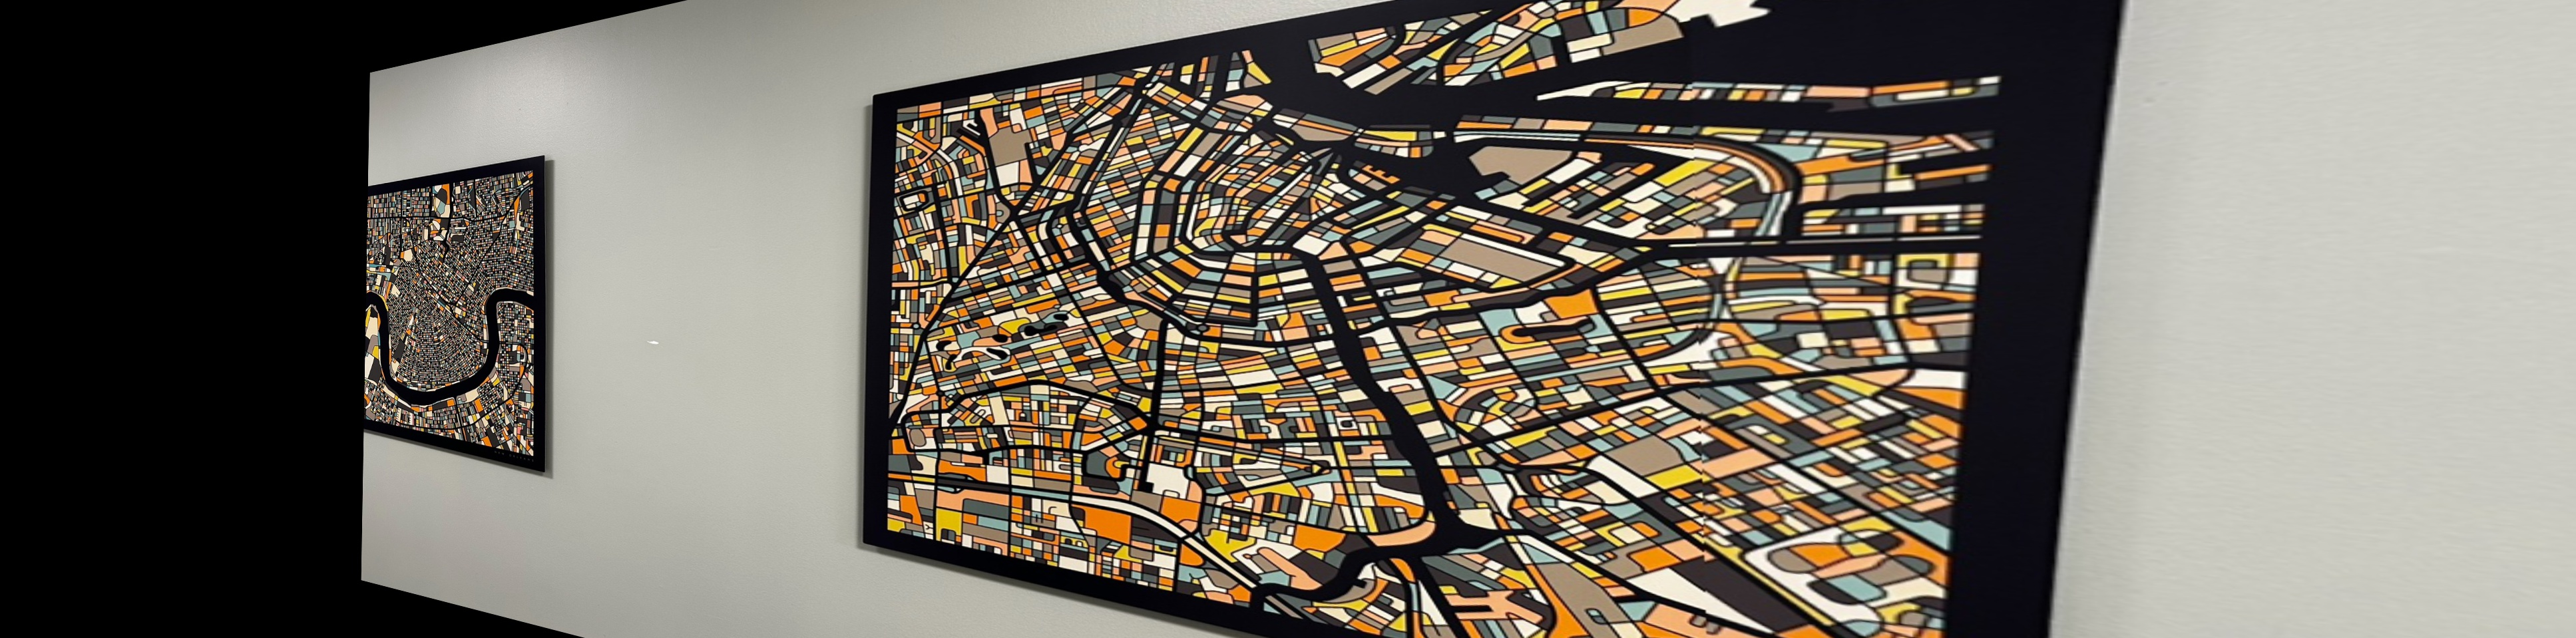
\includegraphics[width=\textwidth]{images/warped-right-3.jpg}
    \caption{Right-Middle Warped to Left}
    \label{fig:cv-desk}
  \end{minipage}
  \hfill
  \begin{minipage}{\textwidth}
    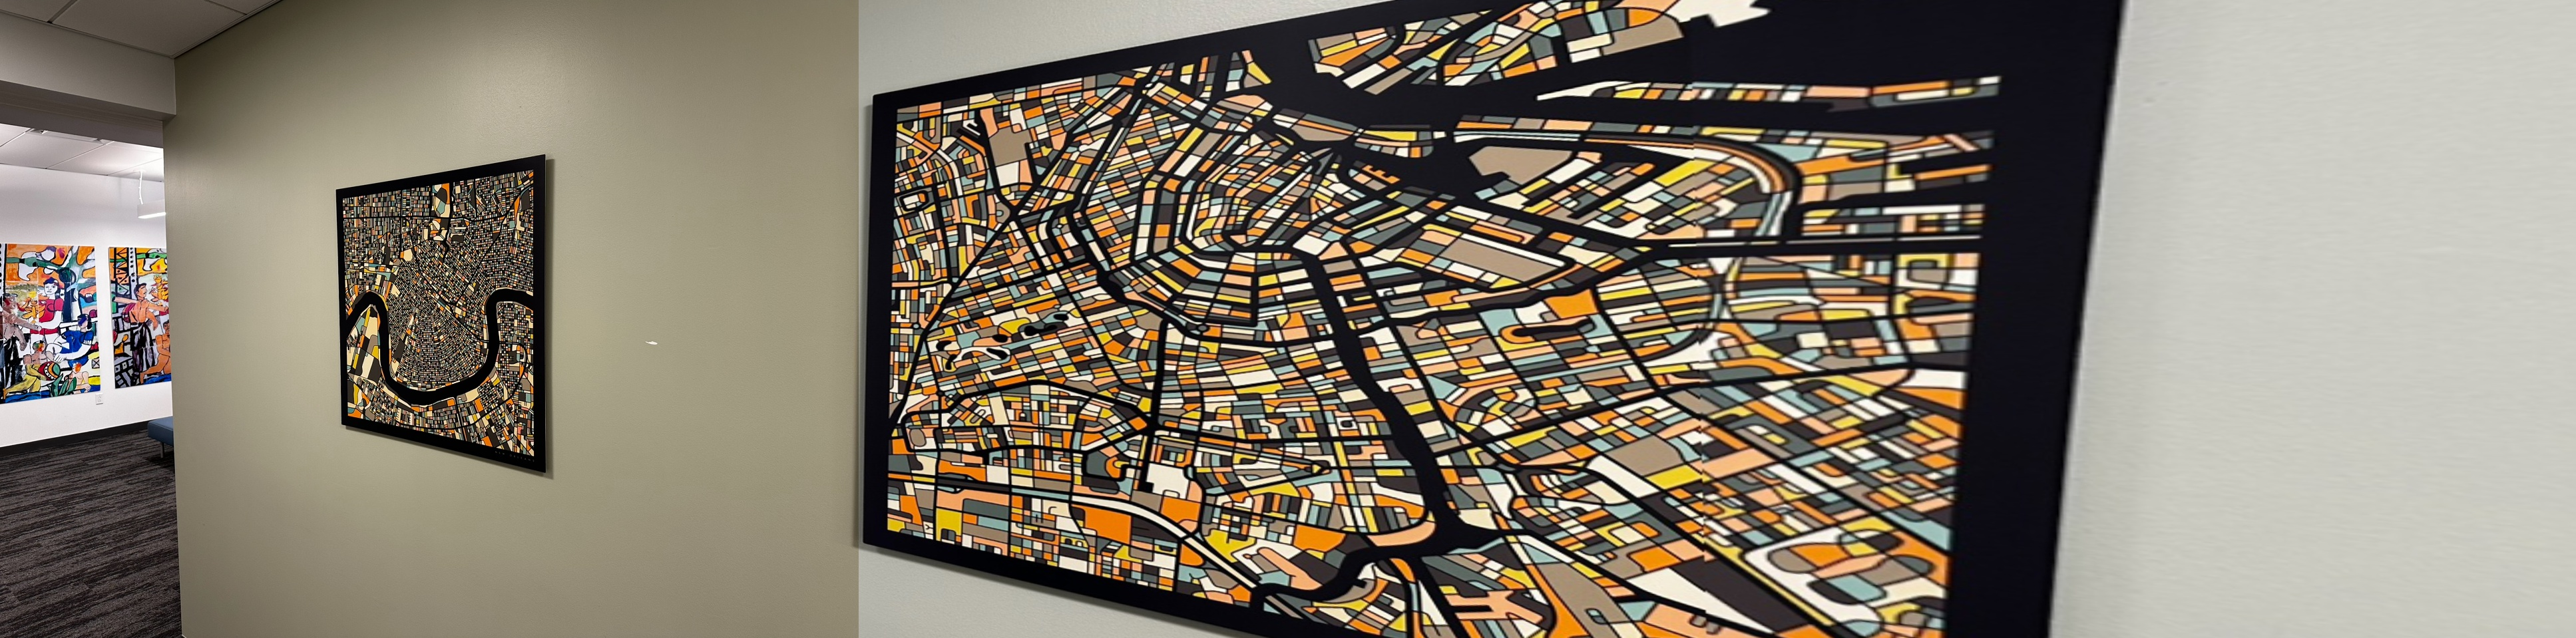
\includegraphics[width=\textwidth]{images/panorama-3.jpg}
    \caption{Left + (Middle + Right)}
    \label{fig:hp-desk}
  \end{minipage}
\end{figure}

